\chapter{Prezentarea aplicației}

OfOps este o aplicație WEB concepută pentru simplificarea procesului de rezervare a diferitelor resurse dintr-un mediu de lucru. Indiferent dacă aveți nevoie să vă asigurați un loc de parcare, să rezervați un birou pentru o anumită perioadă de timp sau o sală de ședință, OfOps vine în ajutorul tău!

\section{Pagina principală și mențiuni generale}

Pagina principală este cea care întâmpină utilizatorul în momentul în care navighează pentru prima oară pe ea. Aceasta oferă opțiuni limitate utilizatorului și anume cele de \textbf{Login} și \textbf{Create an account}.

\begin{figure}[!htb]
    \centering
    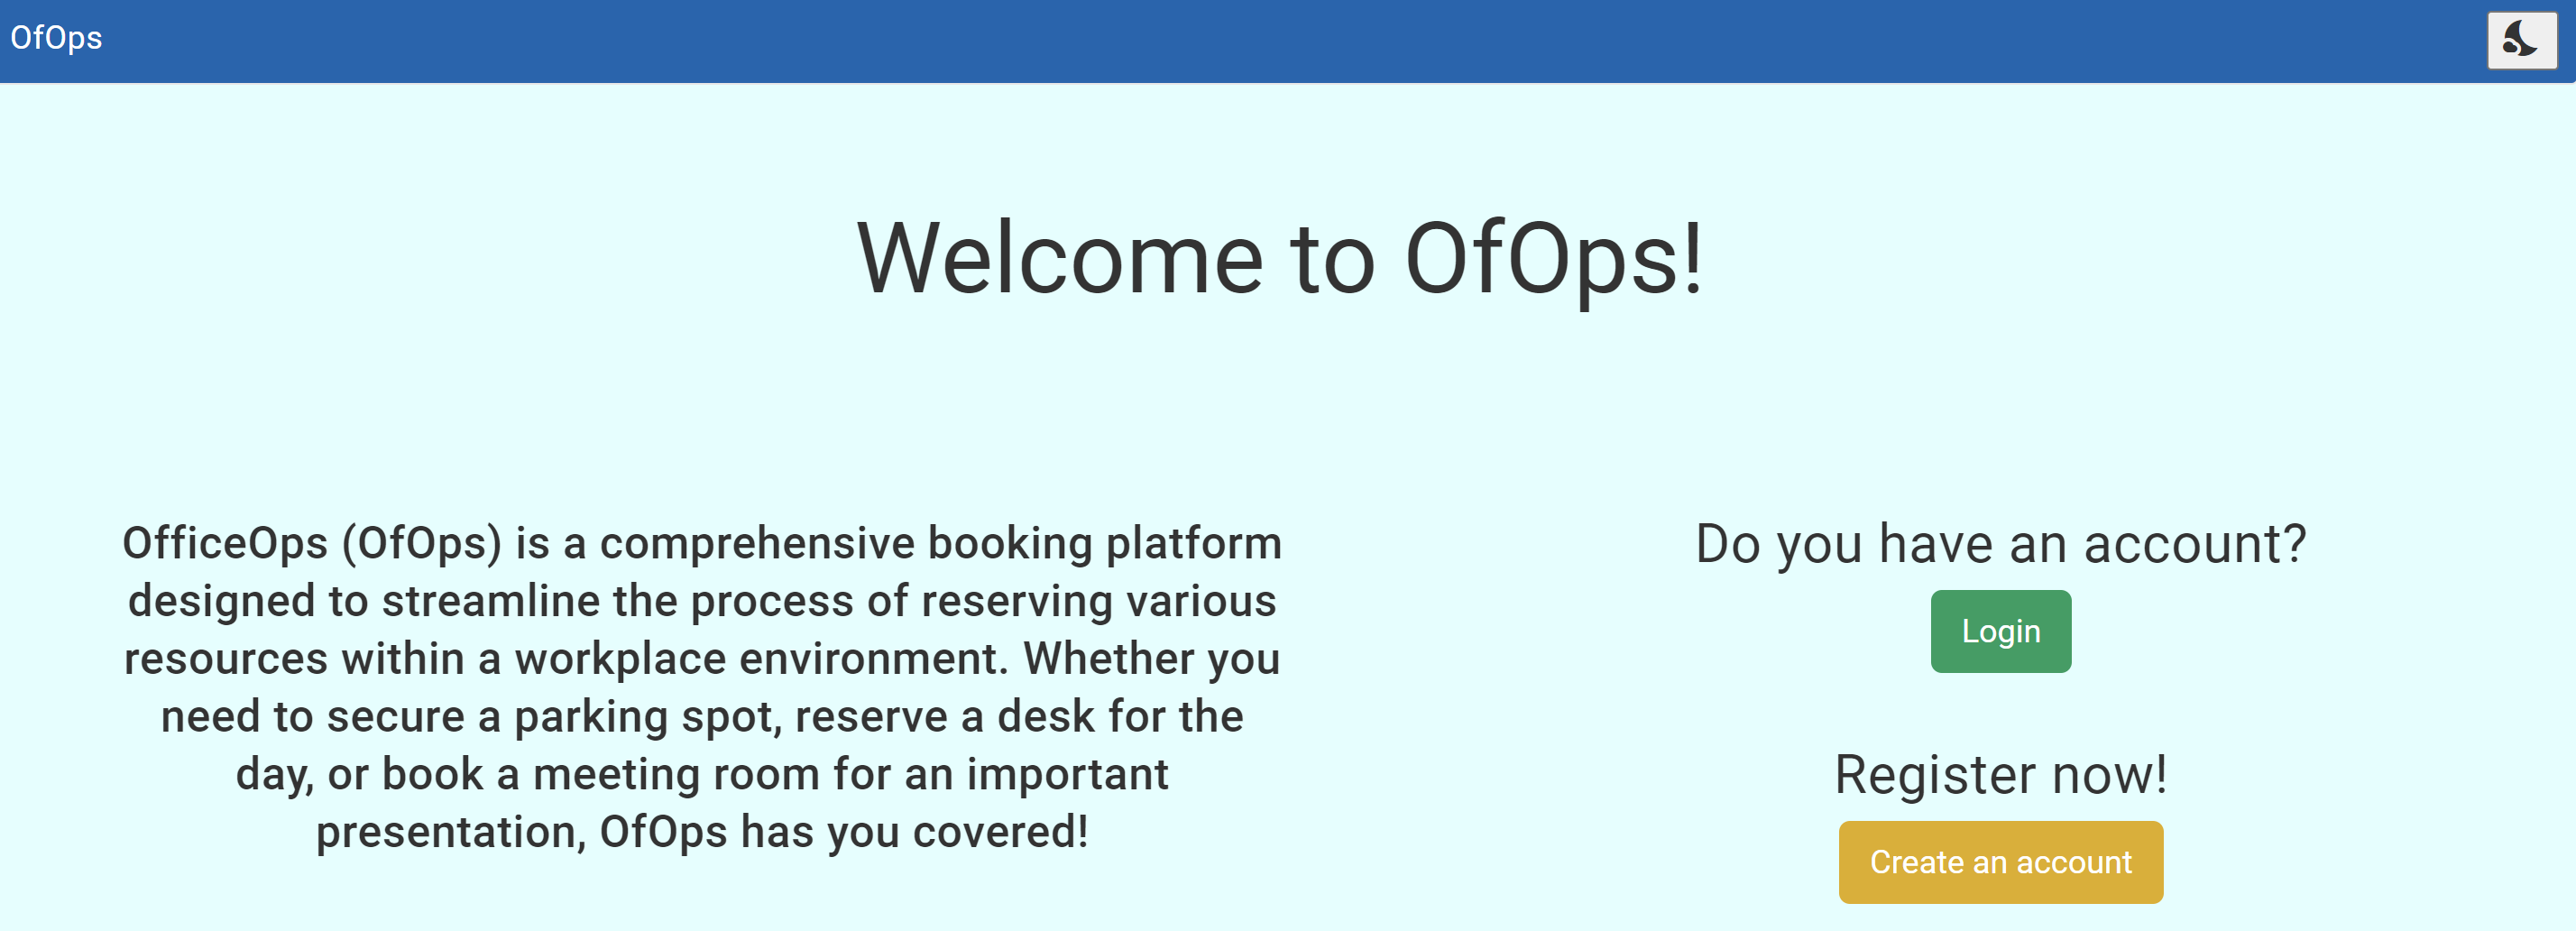
\includegraphics[width=0.9\linewidth]{images/pagina-nelogat.png}
    \caption{Pagina principală}
    \label{fig:principal}
\end{figure}

De asemenea, OfOps dispune și de varianta pentru dark mode. Această opțiune, cunoscută și sub denumirea de night mode, a devenit populară în ultimii ani, mai exact, din anul 2019 în care Google a introdus-o pe Android OS, fapt ce i-a făcut pe toți giganții din industria IT să-i urmeze modelul.\cite{citation9} Posibilitatea utilizatorului de alege modul de navigare pe aplicație denotă prioritizarea dorințelor acestuia, rezultâand, astfel, o experiență mult mai plăcută pentru el. Schimbarea la dark mode se realizează prin apăsarea butonului din dreapta sus a paginii.

\begin{figure}[!htb]
    \centering
    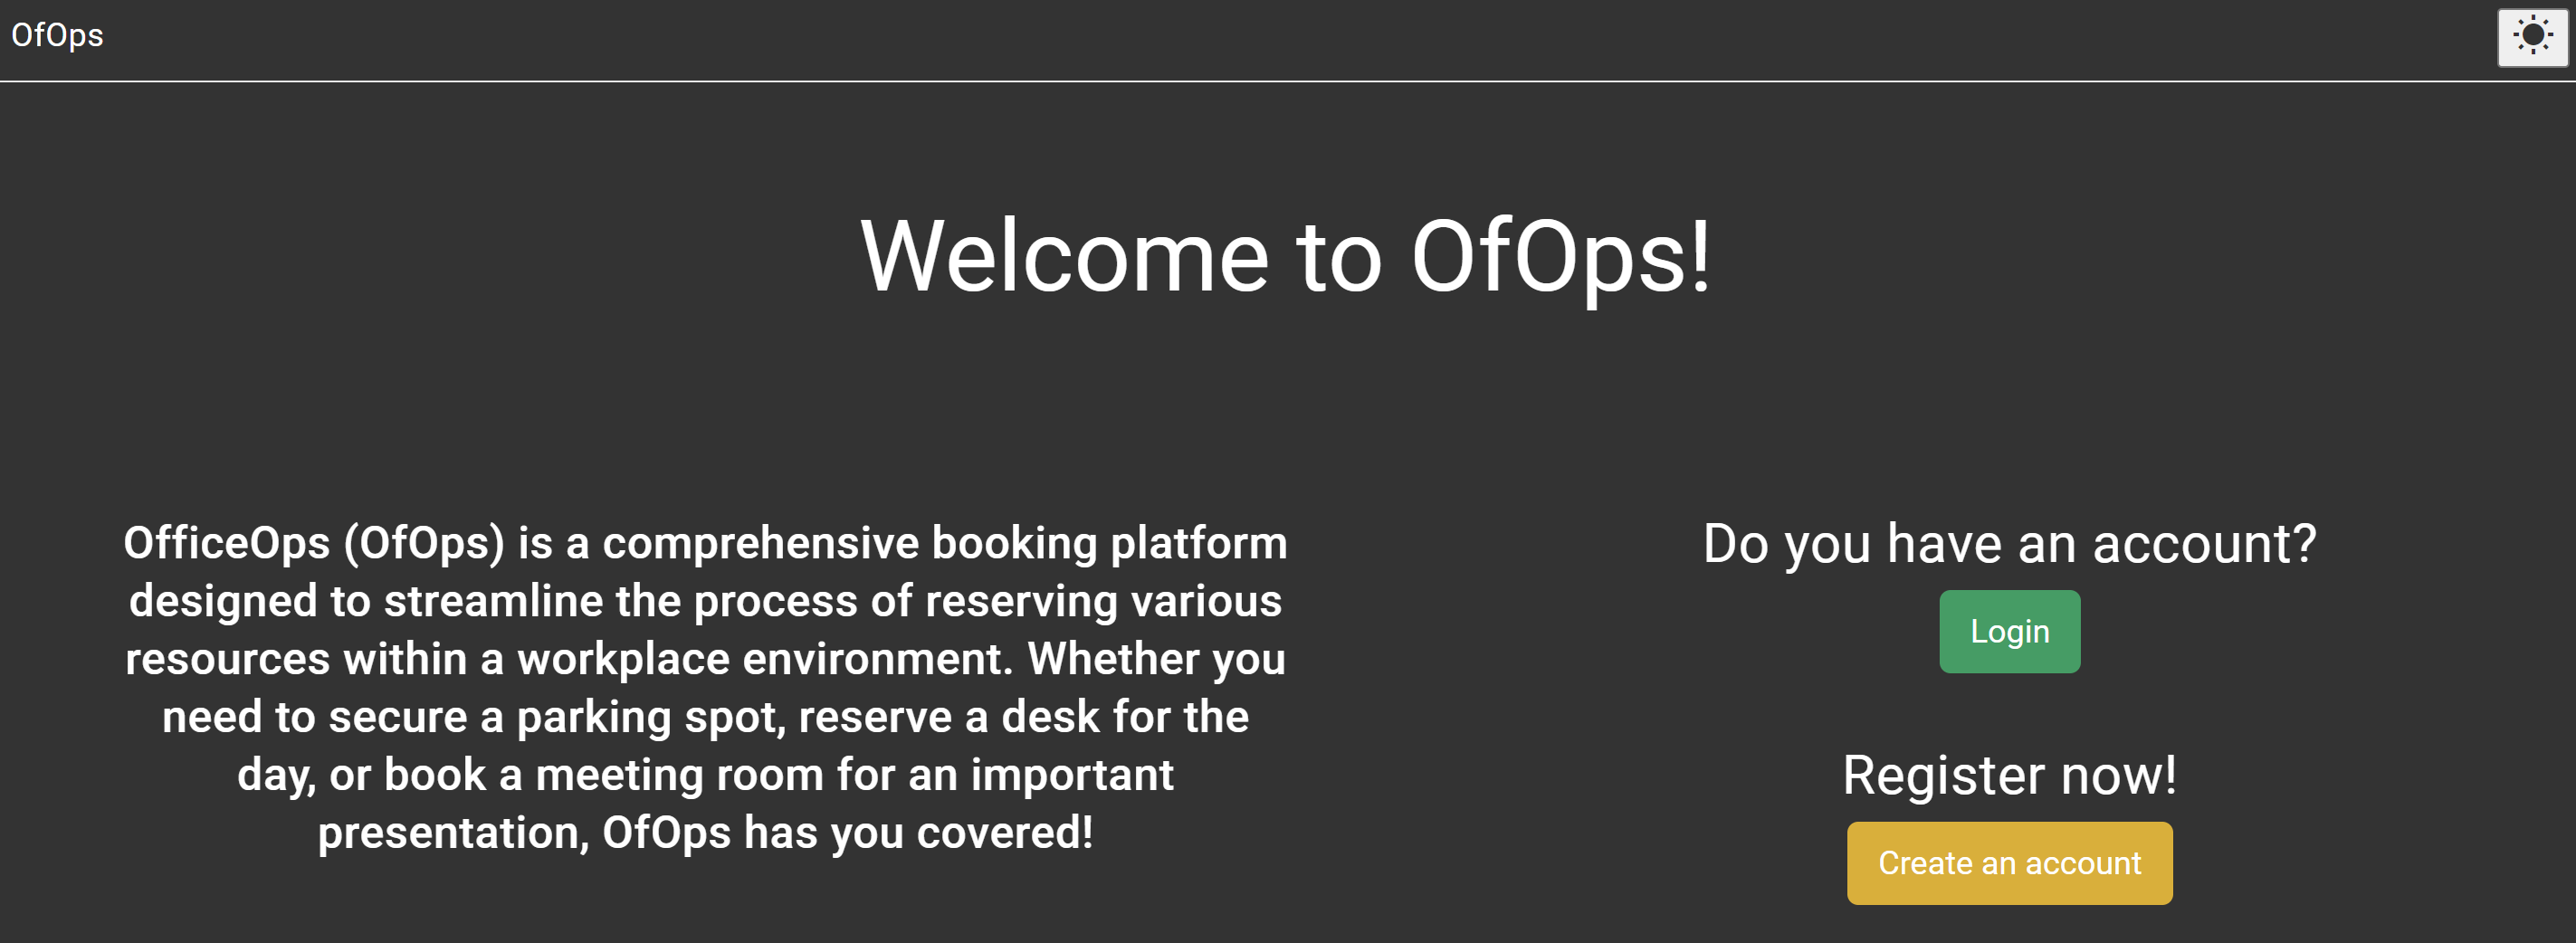
\includegraphics[width=0.9\linewidth]{images/dark.png}
    \caption{Dark mode}
    \label{fig:dark}
\end{figure}

\section{Pagina de înregistrare a unui utilizator}

Pagina de înregistrare a unui utilizator este disponibilă în momentul click-ului pe butonul \textbf{Create an account} din pagina principală. Utilizatorul este redirecționar către formularul de creare a unui cont.  

\begin{figure}[!htb]
    \centering
    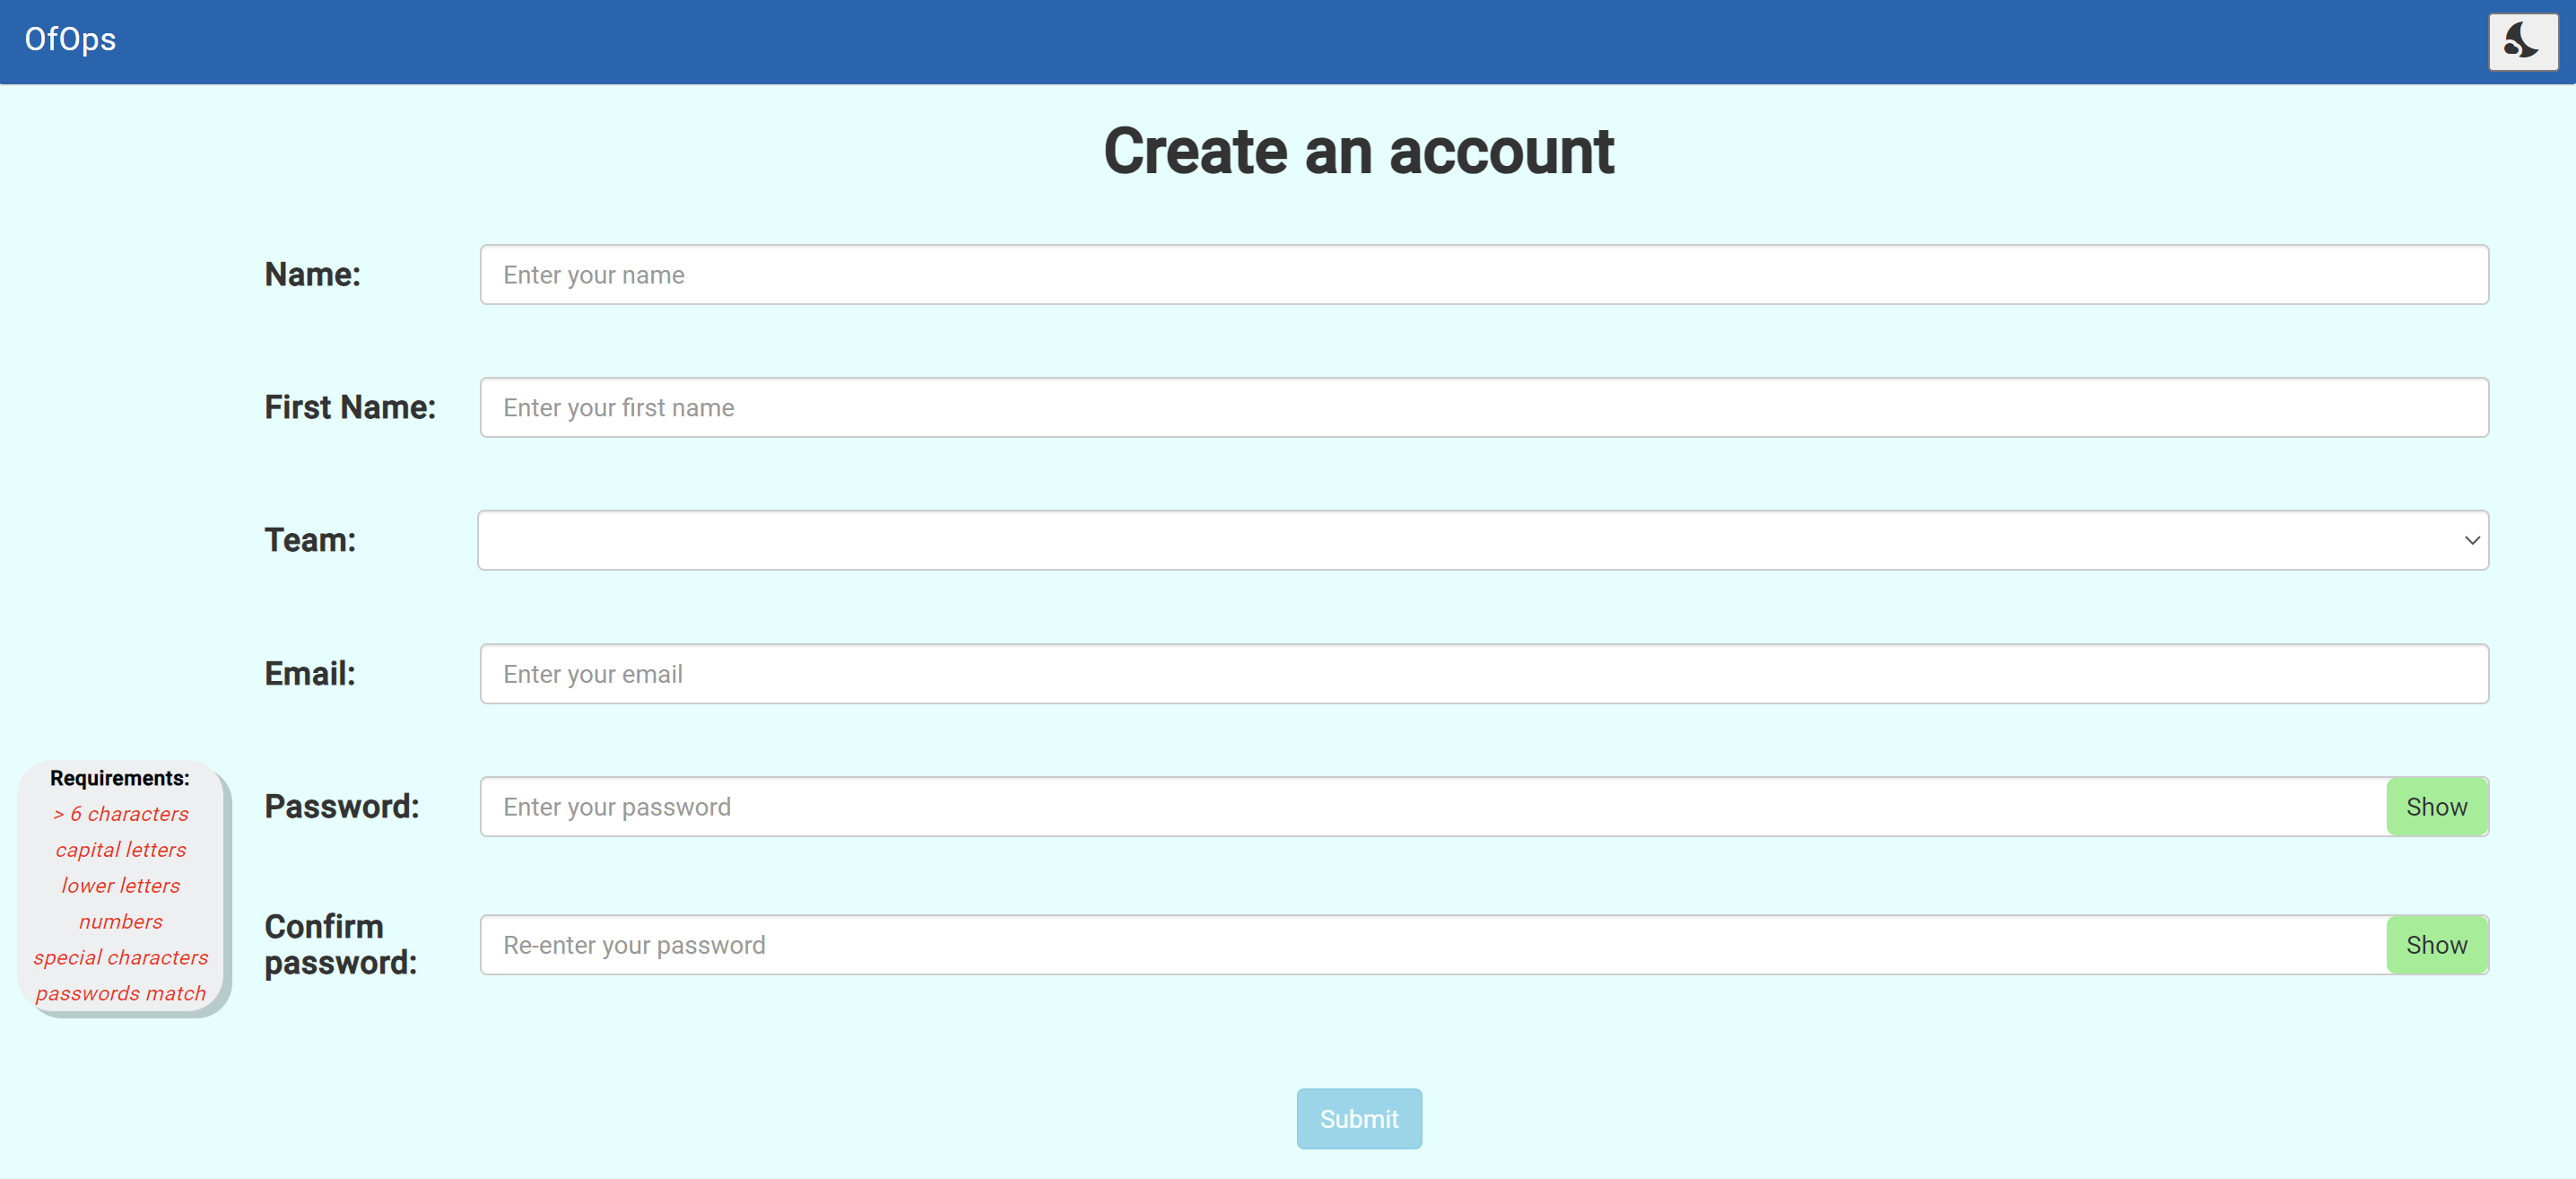
\includegraphics[width=0.9\linewidth]{images/inregistrare.png}
    \caption{Înregistrarea pe OfOps}
    \label{fig:inregistrare}
\end{figure}

Crearea unui cont se realizează pein completarea tuturor câmpurilor. Acestea au implementate validări pe care dacă user-ul nu le îndeplinește va duce la inactivarea butonului de submit. În caz contrar, butonul se va activa. De asemenea, există un set de reguli pentru parolă, astfel încât aceasta să fie cât mai greu de spart. Utlizitatorul are posibilitatea să își vadă parola în cazul în care nu se potrivește cu cea trecută la \textbf{Confirm password}.

\newpage

\begin{figure}[!htb]
    \centering
    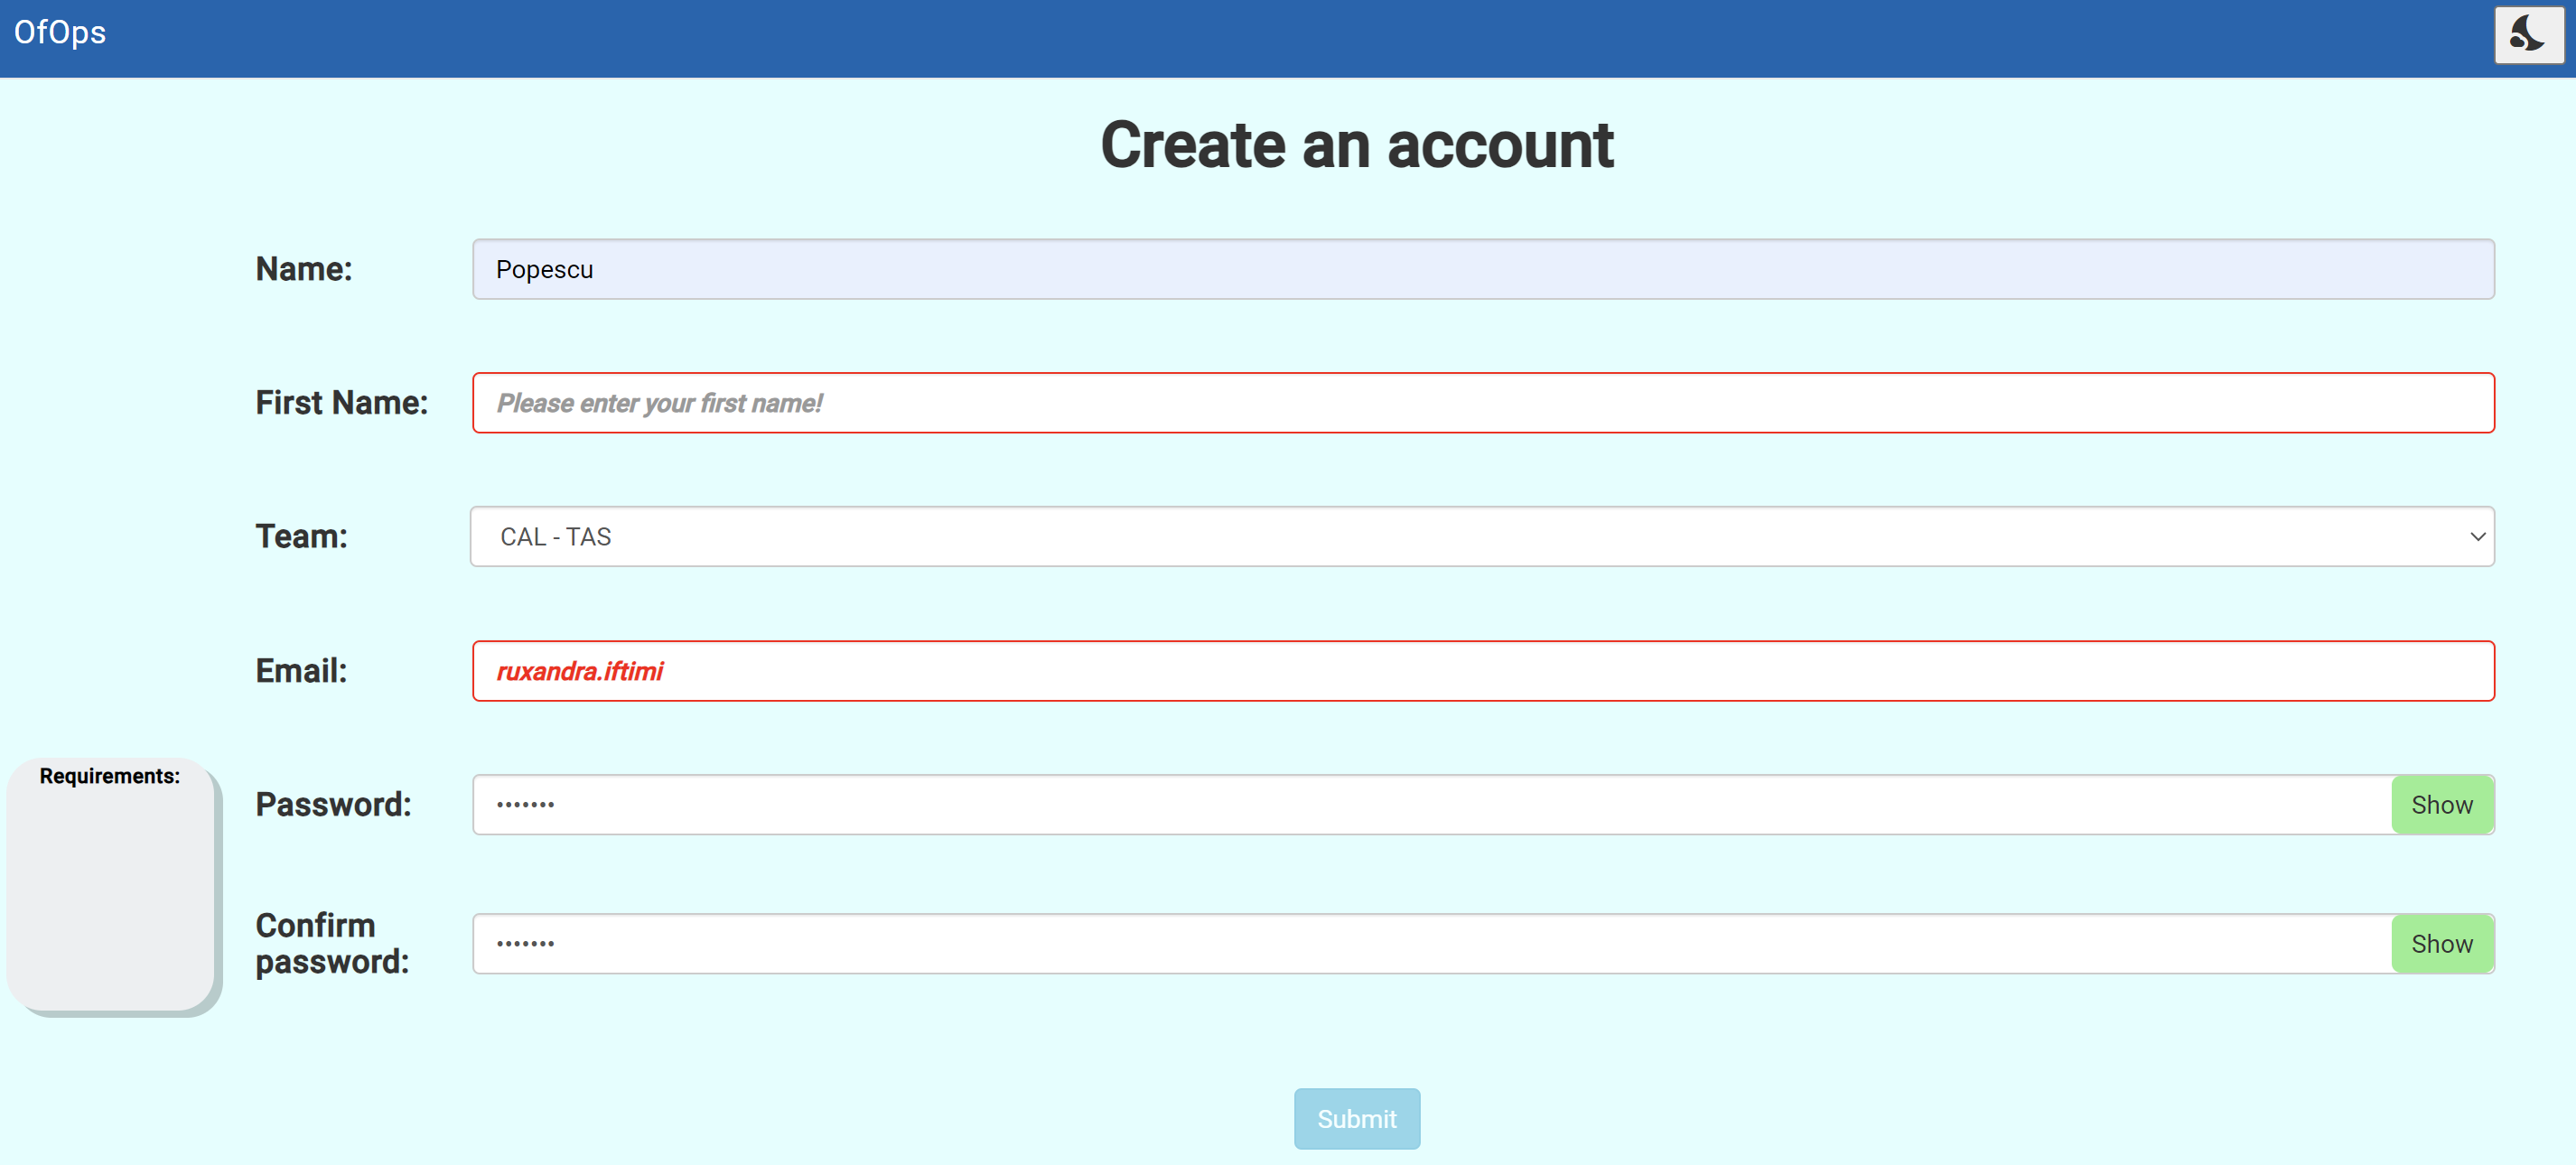
\includegraphics[width=0.9\linewidth]{images/greseli.png}
    \caption{Validările câmpurilor nu sunt respectate}
    \label{fig:greseli}
\end{figure}

La apăsarea butonului de \textbf{Submit}, user-ul va fi redirecționat către pagina de \textbf{Sign in}, primind un pop-up legat de viitoarea autentificare în aplicație.  

\begin{figure}[!htb]
    \centering
    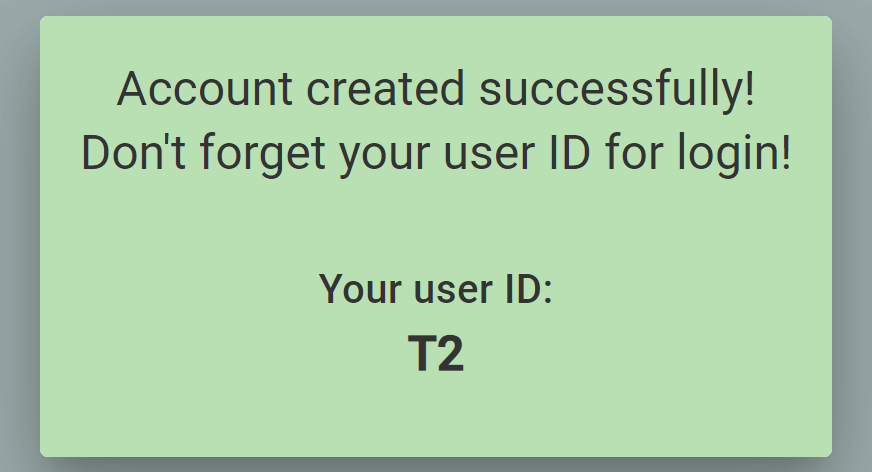
\includegraphics[width=0.9\linewidth]{images/autentf.png}
    \caption{Înregistrare reușită}
    \label{fig:autentf}
\end{figure}

\section{Pagina de sign in}

\section{Rezervarea unui loc}

\section{Rezervarea unei săli de ședință}

\section{Rezervările mele}




